\documentclass[dvipdfmx,a4paper]{jsarticle}
    \pagestyle{plain}
    \usepackage{amsmath}
    \usepackage{amsthm}
    \usepackage{amssymb}
    \usepackage{graphicx}
    \usepackage{tikz}
    \usepackage{tkz-euclide}
    \usepackage{here}
    \usepackage{cancel}

    \usetikzlibrary{angles}

    \newcommand{\R}{\mathbb{R}}
    \newcommand{\C}{\mathbb{C}}
    \newcommand{\Z}{\mathbb{Z}}
    \newcommand{\N}{\mathbb{N}}
    \newcommand{\Q}{\mathbb{Q}}
    \newcommand{\Lra}{\Leftrightarrow}
    \newcommand{\al}{\alpha}
    \newcommand{\be}{\beta}
    \newcommand{\ga}{\gamma}
    \newcommand{\om}{\omega}
    \newcommand{\De}{\Delta}
    \newcommand{\oraw}{\overrightarrow}
    \newcommand{\posv}[1]{\overrightarrow{\mathrm{#1}}}
    \newcommand{\comb}[2]{{}_{#1}\mathrm{C}_{#2}}
    \newcommand{\perm}[2]{{}_{#1}\mathrm{P}_{#2}}
    \newcommand{\bs}{\backslash}
    \newcommand{\2}{I\hspace{-1pt}I}
    \newcommand{\3}{I\hspace{-1pt}I\hspace{-1pt}I}

    \newtheorem{cs}{Case}
    \newtheorem{cas}{Case}
    \newtheorem{case}{Case}
    \newtheorem{apf}{別解}
    \newtheorem{anpf}{別解}

    \usetikzlibrary{calc}
    \title{2023年度京大数学(文系)の解答}
    \author{tt0801}
    \date{\today}
    
    \begin{document}
    \maketitle
    \section{大問1}
    \subsection{問題}
    次の各問に答えよ. 

    \begin{itemize}
        \item [問1] \quad $n$ を自然数とする. 1個のさいころを $n$ 回投げるとき, 出た目の積が 5 で割り切れる確率を求めよ. 
        \item [問2] \quad 次の式の分母を有理化し, 分母に 3 乗根の記号が含まれない式として表せ. 
            \[
                \frac{55}{2 \sqrt[3]{9} + \sqrt[3]{3} + 5}
            \]
    \end{itemize}

    \subsection{解答}
    \begin{itemize}
        \item [問1] \quad 出た目の積が5で割り切れる事象の余事象は, いずれの目も5でない事象であり, 
            その確率は, $\left(\dfrac{5}{6}\right)^n$である. よって, 求める確率は, $1-\left(\dfrac{5}{6}\right)^n$
            である. 
        \item [問2] \quad $a=2 \sqrt[3]{9}$, $b=\sqrt[3]{3}$, $c=5$とおく. 
        \begin{align*}
            (a + b +c)(a^2 + b^2 + c^2 - ab -bc -ca) &= a^3 + b^3 + c^3 -3abc \\
            &= 72 + 3 + 125 -90 \\
            &= 110
        \end{align*}
        である. よって, 
        \begin{align*}
            a^2 + b^2 + c^2 - ab -bc -ca 
            &= 12 \sqrt[3]{3} + \sqrt[3]{9} + 25 - 6 -5\sqrt[3]{3} - 10\sqrt[3]{9} \\
            &= -9 \sqrt[3]{9} + 7 \sqrt[3]{3} + 19
        \end{align*}
        を分母分子にかけて, 
        \begin{align*}
            \dfrac{55}{2 \sqrt[3]{9} + \sqrt[3]{3} + 5}
            &= \dfrac{55(-9 \sqrt[3]{9} + 7 \sqrt[3]{3} + 19)}{110} \\
            &= \dfrac{-9 \sqrt[3]{9} + 7 \sqrt[3]{3} + 19}{2}
        \end{align*}
        と有理化できる. 
    \end{itemize}

    \subsection{別解}
    \begin{itemize}
        \item [問2] $x,y,z$を実数とする. 
        \begin{align*}
            (2 \sqrt[3]{9} + \sqrt[3]{3} + 5)(x \sqrt[3]{9} + y\sqrt[3]{3} + z) 
            &= (5x+y+2z)\sqrt[3]{9} + (6x + 5y + z)\sqrt[3]{3} + (3x + 6y + 5z)
        \end{align*}
        である. $5x+y+2z=6x + 5y + z=0$を$y,z$について解くと, 
        \begin{equation*}
            y = -\dfrac{7}{9}x, \quad z = - \dfrac{19}{9}x
        \end{equation*}
        である. そこで, $(x,y,z)=(-9,7,19)$とおけば, 
        \begin{align*}
            (2 \sqrt[3]{9} + \sqrt[3]{3} + 5)(-9 \sqrt[3]{9} + 7\sqrt[3]{3} + 19) 
            &= 3\cdot (-9) + 6\cdot 7 + 5 \cdot 19 \\
            &= 110
        \end{align*}
        である. 以上より, 
        \begin{align*}
            \dfrac{55}{2 \sqrt[3]{9} + \sqrt[3]{3} + 5}
            &= \dfrac{55(-9 \sqrt[3]{9} + 7 \sqrt[3]{3} + 19)}{110} \\
            &= \dfrac{-9 \sqrt[3]{9} + 7 \sqrt[3]{3} + 19}{2}
        \end{align*}
        と有理化できる. 
    \end{itemize}



    \subsection{解説}
    次の因数分解は導出できるようにしよう. 
    \[
        a^3 + b^3 + c^3 -3abc = (a + b +c)(a^2 + b^2 + c^2 - ab -bc -ca).
    \]
    問2は, この因数分解を知らなくても別解のように有理化を導くことができる. しかも, 
    別解の方法は原理的に$n$乗根の場合にも対応している. 
    
    \section{大問2}
    \subsection{問題}
    空間内の4点 O, A, B, Cは同一平面上にないとする. 点D, P, Qを次のように定める. 
    点Dは$\posv{OD} = \posv{OA} + 2\posv{OB} + 3\posv{OC}$ を満たし,   
    点Pは線分OAを$1 : 2$に内分し, 点Qは線分OBの中点である. さらに,   
    直線OD上の点Rを, 直線QRと直線PCが交点を持つように定める.   

    このとき, 線分ORの長さと線分RDの長さの比$\mathrm{OR} : \mathrm{RD}$を求めよ. 
    \subsection{解答}
    点Pは線分OAを$1 : 2$に内分するので, $\posv{OP} = \dfrac{1}{3}\posv{OA}$である. 
    点Qは線分OBの中点なので, $\posv{OQ} = \dfrac{1}{2}\posv{OB}$である. 
    点Rは直線OD上にあるので, 実数$s$を用いて, 
    \begin{align*}
        \posv{OR} &= s \posv{OD} \\
        &= s\posv{OA} + 2s\posv{OB} + 3s\posv{OC}
    \end{align*}
    と表せる. 直線QRと直線PCの交点Sは, 直線QR上にあるので実数$t$を用いて, 
    \begin{align*}
        \posv{OS} &= t \posv{OR} + (1-t) \posv{OQ}\\
        &= st\posv{OA} + \left(2st-\dfrac{1}{2}t+\dfrac{1}{2}\right)\posv{OB} + 3st\posv{OC} \\
    \end{align*}
    と表せる. また, 直線PC上にもあるので, 実数$u$を用いて, 
    \begin{align*}
        \posv{OS} &= u \posv{OP} + (1-u) \posv{OC}\\
        &= \dfrac{1}{3}u \posv{OA} + (1-u) \posv{OC}
    \end{align*}
    と表せる. 
    
    空間内の4点 O, A, B, Cは同一平面上にないので, $\posv{OA},\posv{OB},\posv{OC}$は一次独立だから, 
    上記の二通りの$\posv{OS}$の表記は一致する. すなわち, 
    \begin{align*}
        st = \dfrac{1}{3}u, \quad 2st-\dfrac{1}{2}t+\dfrac{1}{2} = 0, \quad 3st = 1-u
    \end{align*}
    である. 一つ目と二つ目の等式より, $3st=u=1-u$なので, $u = \dfrac{1}{2}$, $st = \dfrac{1}{6}$
    である. これを二つの目の等式に代入して, $t = \dfrac{5}{3}$, $s = \dfrac{1}{10}$を得る. 

    以上より, $\posv{OR} =  \dfrac{1}{10}\posv{OD}$であるので, 点Rは辺ODを$1:9$に内分する点である. 
    すなわち, $\mathrm{OR} : \mathrm{RD} = 1:9$である. 

    \subsection{別解}
    点Pは線分OAを$1 : 2$に内分するので, $\posv{OP} = \dfrac{1}{3}\posv{OA}$である. 
    点Qは線分OBの中点なので, $\posv{OQ} = \dfrac{1}{2}\posv{OB}$である. 
    $\posv{OA}, \posv{OB}, \posv{OC}$は一次独立なので, $\posv{OP}, \posv{OQ}, \posv{OC}$も
    一次独立である. 特に, 三点P, Q, Cは同一直線上に存在しないので, P, Q, Cを通る平面は唯一つ定まる. 
    点Rは直線OD上にあるので, 実数$s$を用いて, 
    \begin{align*}
        \posv{OR} &= s \posv{OD} \\
        &= s\posv{OA} + 2s\posv{OB} + 3s\posv{OC} \\
        &= 3s \cdot \dfrac{1}{3}\posv{OA} + 4s \cdot \dfrac{1}{2}\posv{OB} + 3s\posv{OC} \\
        &= 3s \posv{OP} + 4s\posv{OQ} + 3s\posv{OC}
    \end{align*}
    と表せる. 直線QRと直線PCが交点を持つ時, 点Rは平面PQC上に存在するので, 
    \begin{equation*}
        3s + 4s + 3s = 1
    \end{equation*}
    である. すなわち, $s = \dfrac{1}{10}$である. 

    以上より, $\posv{OR} =  \dfrac{1}{10}\posv{OD}$であるので, 点Rは辺ODを$1:9$に内分する点である. 
    すなわち, $\mathrm{OR} : \mathrm{RD} = 1:9$である. 
    
    \subsection{解説}
    一次独立なベクトル$\posv{OA},\posv{OB},\posv{OC}$に着目して表せばよい. 

    \section{大問3}
    \subsection{問題}
    \begin{itemize}
        \item [(1)] $\cos 2\theta$と$\cos 3\theta$を$\cos \theta$の式として表せ. 
        \item [(2)] 半径1の円に内接する正五角形の一辺の長さが1.15より大きいか否かを理由を付けて判定せよ. 
    \end{itemize}

    \subsection{解答}
    \begin{itemize}
        \item [(1)] 二倍角の公式, 三倍角の公式より, 
        \begin{align*}
            \cos 2\theta &= 2\cos^2 \theta -1, \\
            \cos 3\theta &= 4\cos^3 \theta -3 \cos \theta.
        \end{align*}
        \item [(2)] 半径1の円に内接する正五角形の一辺の長さを$h$とすると, 
        図より
        \begin{equation*}
            h = 2 \sin \dfrac{\pi}{5}
        \end{equation*}
        である. 
        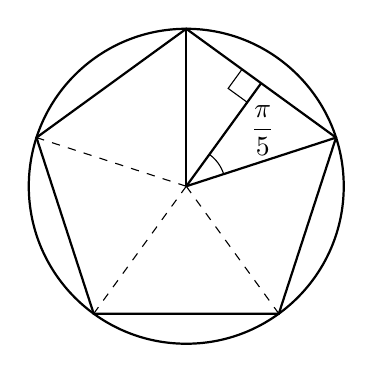
\begin{tikzpicture}
            % Draw the unit circle
            \draw[thick] (0,0) circle(2);
        
            % Define the vertices of the pentagon
            \coordinate (O) at (0,0);
            \foreach \i in {1,2,3,4,5} {
                \coordinate (P\i) at ({2*cos(90 + \i*360/5)}, {2*sin(90 + \i*360/5)});
            }
            \coordinate (M) at ({cos(90 - 360/5)}, {1 + sin(90 - 360/5)});
        
            % Draw the pentagon
            \draw[thick] (P1) -- (P2) -- (P3) -- (P4) -- (P5) -- cycle;
        
            % Draw radius lines to vertices
            \foreach \i in {1,2,3} {
                \draw[dashed] (0,0) -- (P\i);
            }
            \draw[thick] (0,0) -- (P4);
            \draw[thick] (0,0) -- (P5);
            \draw[thick] (0,0) -- (M);

            \pic[draw, -, "$\dfrac{\pi}{5}$", angle radius=0.5cm, angle eccentricity=2.4] {angle=P4--O--M};
            \pic[draw, angle radius=0.3cm] {right angle=P5--M--O};

        \end{tikzpicture}

        \begin{align*}
            \sin 5\theta 
            &= \sin (2\theta + 3\theta) \\
            &= \sin 2\theta \cos 3\theta + \cos 2\theta \sin 3\theta \\
            &= 2\sin \theta \cos \theta (4\cos^3 \theta -3 \cos \theta) + (2\cos^2 \theta -1)(-4 \sin^3 \theta + 3\sin \theta) \\
            &= \sin \theta \left\{2\cos^2 \theta (4\cos^2 \theta -3)+ (2\cos^2 \theta -1)(-4 \sin^2 \theta + 3)\right\} \\
            &= \sin \theta \left[2(1-\sin^2\theta)\left\{4(1-\sin^2\theta)  -3\right\}+ \left\{2(1-\sin^2\theta)  -1\right\}(-4 \sin^2 \theta + 3)\right] \\
            &= \sin \theta \left\{2(1-\sin^2\theta)(-4\sin^2 \theta +1)+ (-2\sin^2 \theta +1)(-4 \sin^2 \theta + 3)\right\} \\
            &= \sin \theta (16\sin^4\theta - 20 \sin^2 \theta +5)
        \end{align*}
        である. $\theta = \dfrac{\pi}{5}$を代入すると, 左辺は$\sin 5\theta = \sin \pi =0$なので, 
        $\sin \dfrac{\pi}{5} >0$に注意すると, 
        \begin{align*}
            16\sin^4\dfrac{\pi}{5} - 20 \sin^2\dfrac{\pi}{5}  +5 = 0
        \end{align*}
        である. すなわち, $\alpha = \sin \dfrac{\pi}{5}$とおくと, $\alpha^2$は, $16x^2 -20x + 5$の
        根である. 同様にして, $\beta = \sin \dfrac{2\pi}{5}$とおくと, 
        $\beta^2$も$16x^2 -20x + 5$の根である. $0<\dfrac{\pi}{5} < \dfrac{2\pi}{5}<\dfrac{\pi}{2}$より, 
        $0<\alpha < \beta$に注意すると, $16x^2 -20x + 5=0$を解いて, 
        \begin{align*}
            \alpha^2 = \dfrac{5-\sqrt{5}}{8}, \quad \beta^2 = \dfrac{5+\sqrt{5}}{8}
        \end{align*}
        を得る. $h=2\alpha$より, 
        \begin{align*}
            h^2 - \left(\dfrac{23}{20}\right)^2 &= 4\alpha ^2 - \left(\dfrac{23}{20}\right)^2\\
            &= \dfrac{5-\sqrt{5}}{2} - \dfrac{529}{400} \\
            &= \dfrac{471-200\sqrt{5}}{400} \\
            & > 0
        \end{align*}
        だから, $h > \dfrac{23}{20} = 1.15$である. 

        以上より, 半径1の円に内接する正五角形の一辺の長さは, 1.15よりも大きい. 
    \end{itemize}

    \subsection{別解}
    \begin{itemize}
        \item [(2)] 半径1の円に内接する正五角形の一辺の長さを$h$とすると, 
        図より
        \begin{align*}
            h &= 2 \sin \dfrac{\pi}{5} \\
            &= 2 \sqrt{1 - \cos^2 \dfrac{\pi}{5}}
        \end{align*}
        である(図は解答と同じなので省略). 
        $\theta = \dfrac{\pi}{5}$とおくと, $5\theta = \pi$なので, $\cos 2\theta = \cos (\pi - 3\theta) = - cos 3\theta$
        である. (1)を踏まえて, 
        \begin{equation*}
            2\cos^2 \theta -1 = - \left(4\cos^3 \theta -3 \cos \theta \right)
        \end{equation*}
        である. この式を整理して, 
        \begin{equation*}
            (\cos \theta + 1)(4 \cos^2 \theta -2 \cos \theta -1) = 0
        \end{equation*}
        を得る. ゆえに, $\cos \theta$の値は
        \begin{equation*}
            \cos \theta = -1, \dfrac{1 \pm \sqrt{5}}{4}
        \end{equation*}
        のいずれかである. $0 < \theta = \dfrac{\pi}{5} < \dfrac{\pi}{2}$なので, 
        $\cos \theta > 0$より, 
        \begin{equation*}
            \cos \theta = \dfrac{1 + \sqrt{5}}{4}
        \end{equation*}
        と定まる. 
        この時, 
        \begin{align*}
            h^2 - \left(\dfrac{23}{20}\right)^2 
            &= 4\left(1 - \cos^2 \dfrac{\pi}{5}\right) - \left(\dfrac{23}{20}\right)^2\\
            &= 4\left\{1 - \left(\dfrac{1 + \sqrt{5}}{4} \right)^2\right\}- \left(\dfrac{23}{20}\right)^2 \\
            &= \dfrac{471-200\sqrt{5}}{400} \\
            & > 0
        \end{align*}
        だから, $h > \dfrac{23}{20} = 1.15$である. 
    
        以上より, 半径1の円に内接する正五角形の一辺の長さは, 1.15よりも大きい. 
    
    \end{itemize}


    \subsection{解説}
    $\sin \dfrac{\pi}{5}$の値を評価したいので, $\sin \dfrac{\pi}{5}$が満たす方程式を考えたい. 
    そのため5倍角の公式を導出した. チェビシェフの多項式などの背景知識があると, 解きやすかったかもしれない. 

    余談だが, 解と根の違いは次の通りである. 
    \begin{itemize}
        \item 解は, 方程式や不等式を満たす答えである. すなわち, 何かしら等号($=$)や不等式($>,<,\geq, \leq$)で結ばれる式に対して使用される. 
        \item 根は, 多項式に代入して0となるような値である. すなわち, 多項式$P(x)$について$x=\alpha$が$P(x)=0$
        の解であるならば, $\alpha$は多項式$P(x)$の根である. 

    \end{itemize}

    \section{大問4}
    \subsection{問題}
    数列 $\{a_n\}$ は次の条件を満たしている. 

    \[
    a_1 = 3, \quad a_n = \frac{S_n}{n} + (n-1) \cdot 2^n \quad (n = 2, 3, 4, \ldots)
    \]

    ただし, $S_n = a_1 + a_2 + \cdots + a_n$ である. このとき, 数列 $\{a_n\}$ の一般項を求めよ. 
    \subsection{解答}
    右の条件は, $n=1$でも成立する. 右の条件より, $n\geq 1$で, 
    \begin{align*}
        S_n = n\left\{a_n -(n-1)\cdot 2^n\right\}
    \end{align*}
    である. よって, 任意の自然数$n$に対して, 
    \begin{align*}
        a_{n+1} &= S_{n+1} - S_n \\
                &= (n+1)\left\{a_{n+1} -n\cdot 2^{n+1}\right\} - n\left\{a_n -(n-1)\cdot 2^n\right\} \\
                &= (n+1)a_{n+1} - na_n -n(n+1)2^{n+1} + n(n-1)2^n
    \end{align*}
    が成り立つ. すなわち, 
    \[
        na_{n+1} - na_n = n(n+1)2^{n+1} - n(n-1)2^n
    \]
    なので, 両辺$n\ (n>0)$で割って, 
    \begin{align*}
        a_{n+1} - a_n &= (n+1)2^{n+1} - (n-1)2^n \\
        &= \left\{2(n+1)-(n-1)\right\}2^n \\
        &= (n+3)2^n
    \end{align*}
    を得る. 

    ゆえに, $n$が2以上の自然数の時, 
    \begin{align*}
        a_n &= a_1 + \sum_{k=1}^{n-1} (a_{k+1} - a_k) \\
        &= 3 + \sum_{k=1}^{n-1} (k+3)2^k \\
    \end{align*}
    $\displaystyle b_n = \sum_{k=1}^{n-1} (k+3)2^k$とおくと, 
    \begin{align*}
        b_n &= 2b_n - b_n \\
        &= \sum_{k=1}^{n-1} (k+3)2^{k+1} - \sum_{k=1}^{n-1} (k+3)2^k \\
        &= \sum_{k=2}^{n} (k+2)2^{k} - \sum_{k=1}^{n-1} (k+3)2^k \\
        &= (n+2)2^n - \sum_{k=2}^{n-1} 2^{k} - (1+3)2^1 \\
        &= (n+2)2^n - (2^n-4) - 8 \\
        &= (n+1)2^n -4
    \end{align*}
    である. ゆえに, 
    \begin{align*}
        a_n &= 3 + b_n \\
        &= (n+1)2^n -1
    \end{align*}
    が$n \geq 2$で成立する. これは$n=1$の時も両辺ともに3となり成立する. 

    以上より, 数列 $\{a_n\}$の一般項は, 
    \begin{equation*}
        a_n= (n+1)2^n -1
    \end{equation*}
    である. 

    \subsection{解説}
    とりあえず, $a_n$と$S_n$の関係式$a_{n+1} = S_{n+1} - S_n$に代入すると, 
    解ける漸化式が得られる. 

\end{document}